% Poster get from https://github.com/victorsenam/tcc/blob/master/poster/main.tex

\documentclass[final]{beamer}
\usepackage[size=a1,orientation=portrait,scale=1.3]{beamerposter}

\usepackage[brazil]{babel}
\usepackage[utf8]{inputenc}
\usepackage[T1]{fontenc}
\usepackage{framed,graphicx,xcolor} % for shaded box
\usepackage{mathtools}%
\usepackage{tcolorbox} % Para criar bordas elegantes
\usepackage{graphicx}  % Para incluir imagens
\usepackage{caption}   % Para legendas personalizadas
\usepackage{tikz}
\usetikzlibrary{matrix,shapes,positioning,shadows,trees,patterns}

\usepackage[shortlabels]{enumitem}
\usepackage[numbers]{natbib}
\bibliographystyle{plainnat}
  \def\bibfont{\small}

\sloppy

%----------------------------------------------------------------------------------------
%	SHORTCUTS
%----------------------------------------------------------------------------------------
\newcommand{\B}[1]{\mathbb{#1}}
\newcommand{\Cl}[1]{\ensuremath{\mathcal{#1}}}

\newcommand{\sse}{\Leftrightarrow}
\newcommand{\so}{\Rightarrow}
\newcommand{\se}{\Leftarrow}
\newcommand{\rec}{\leftarrow}

\newcommand{\tdots}{\,.\,.\,}

%----------------------------------------------------------------------------------------
%	BEAMER STYLE
%----------------------------------------------------------------------------------------

\usetheme{poster}
\setbeamercolor{block title}{fg=dblue,bg=white}
\setbeamercolor{block body}{fg=black,bg=white}
\setbeamercolor{block alerted title}{fg=dblue,bg=gray!50}
\setbeamercolor{block alerted body}{fg=black,bg=gray!20}
\setbeamercolor{block prob}{fg=black,bg=white}
\setbeamertemplate{caption}[numbered]

%----------------------------------------------------------------------------------------
%	CUSTOM STYLING
%----------------------------------------------------------------------------------------

\newenvironment<>{prob}{
    \begin{beamercolorbox}[sep=1ex,center,dp={1ex}]{block prob}
    \textcolor{dblue}{\textbf{Problema:}}\itshape
}{\end{beamercolorbox}}

\newcommand\halfcol{\column{.46\textwidth}}
\newcommand\onethirdcol{\column{.31\textwidth}}

\newcommand{\Oh}{\mathrm{O}}

% ?????????
\usepackage{subcaption}

\newcommand*\bolinha[1]{\; \tikz[inner sep=.25ex]\node[circle,draw]{#1}; \;}

%----------------------------------------------------------------------------------------
%	POSTER
%----------------------------------------------------------------------------------------

\title{Rainbow Version of Dirac's Theorem: An Algorithmic Approach}
\author{
  \begin{tabular}{l} % Define uma tabela com alinhamento à esquerda
    Nathan Luiz Bezerra Martins \hspace{200pt} Orientadora: Yoshiko Wakabayashi\\
    Willian Miura Mori
  \end{tabular}
}
\institute{\vspace{10pt}Departamento de Ciência da Computação,\\
Instituto de Matemática e Estatística, Universidade de São Paulo}

\begin{document}
\begin{frame}[fragile]\centering
  \vspace{-40pt}
  \begin{columns}[T]

    % ----------------------------------------------------------------------------------------
    % PRIMEIRA COLUNA
    % ----------------------------------------------------------------------------------------
    \onethirdcol
    \begin{alertblock}{Resumo}
      Dada uma coleção $G = {G_1, G_2, \ldots, G_n}$ de grafos de ordem $n \geq 3$, definidos 
      sobre o mesmo conjunto de vértices e que satisfazem a condição de Dirac para cada 
      $G_i$, existe um $G$-transversal que forma um circuito hamiltoniano, também conhecido
      como Circuito Hamiltoniano Rainbow. Neste trabalho, desenvolvemos um 
      algoritmo eficiente que encontra um Circuito Hamiltoniano Rainbow. Fizemos implementações
      tanto em \texttt{C++} quanto em \texttt{Python} e realizamos testes de desempenho para comparar as duas versões.
      Utilizamos a biblioteca \texttt{manim} para fazer uma animação gráfica do algoritmo.
    \end{alertblock}

    \begin{block}{Conceitos básicos}
        \textbf{Definições principais:}
        \begin{itemize}
          \item Um grafo simples é um grafo não direcionado sem laços e sem arestas múltiplas.
          \item Um \textbf{ciclo hamiltoniano} de $G$ é um ciclo que visita cada vértice de $G$ exatamente uma vez.
          \item $\delta(G)$ é o grau mínimo de um vértice em $G$.
        \end{itemize}
        \vspace{0.5em}
        \textbf{Teorema de Dirac (1952):}
        Se um grafo simples $G$ com $n \geq 3$ vértices tem grau mínimo $\delta(G) \geq \frac{n}{2}$, então $G$ contém um ciclo hamiltoniano.
    \end{block}

    \begin{block}{Versões Rainbow de problemas clássicos}
      \textbf{Definição:}

      A versão rainbow de um problema na teoria dos grafos é uma variação 
      que adiciona a restrição de cores à solução desejada. Nesse contexto, o termo rainbow (arco-íris) refere-se a estruturas em um grafo que utilizam 
      elementos provenientes de diferentes subconjuntos, ou arestas com diferentes rótulos ou cores, 
      garantindo que não haja repetições.
      \vspace{1em}

      \textbf{Teorema de Dirac (\textit{Versão Rainbow}):}

      Dada uma coleção $G = {G_1, G_2, \ldots, G_n}$ de grafos de ordem $n \geq 3$, definidos
      sobre o mesmo conjunto de vértices e que satisfazem a condição de Dirac para cada
      $G_i$, existe um $G$-transversal que forma um circuito hamiltoniano, também conhecido
      como Circuito Hamiltoniano Rainbow.
      Cada grafo $G_i$ pode ser enxergado como se suas arestas fossem coloridas com a cor $i$.
      
      \begin{center}
        \begin{tcolorbox}[
            colframe=black,        % Border color
            colback=white,         % Background color
            coltitle=black,        % Title color (used for caption)
            width=0.6\textwidth,   % Box width, 60% of the text width
            boxrule=0.5mm,         % Border thickness
            arc=4mm,               % Rounded corners
            outer arc=1mm,         % Outer corner rounding
        ]
            \centering
            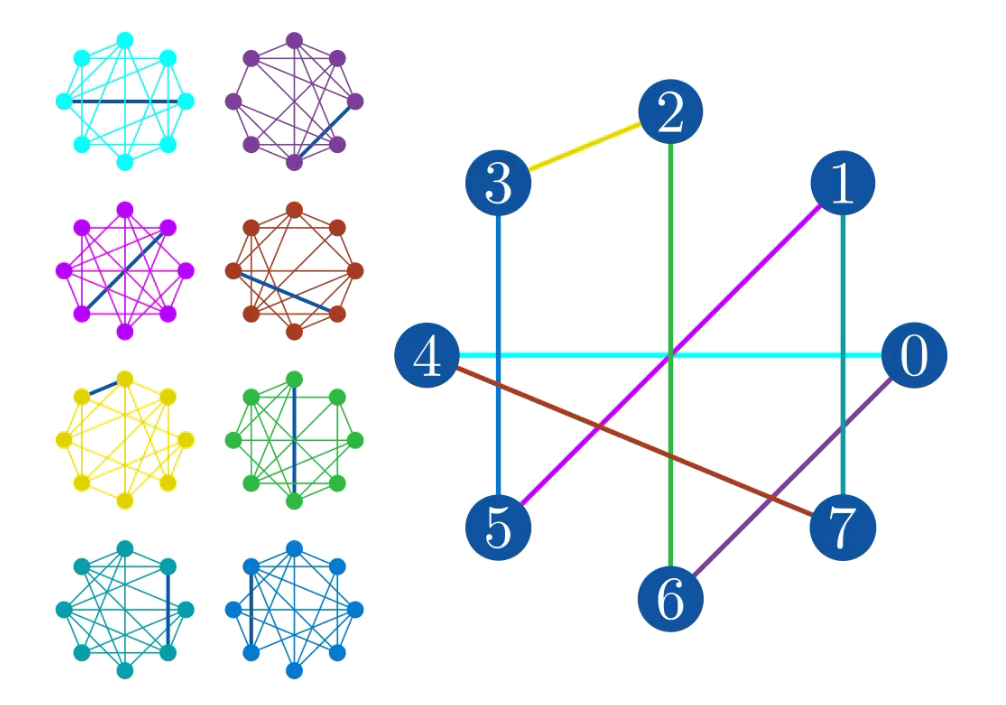
\includegraphics[width=\textwidth]{logos/dirac_rainbow.png}
            \captionof{figure}{Exemplo de um Circuito Hamiltoniano Rainbow para uma coleção de grafos com 8 vértices.}
        \end{tcolorbox}
      \end{center}

      \vspace{1em}
      \textbf{Mais exemplos clássicos:}
      \begin{itemize}
        \item \textbf{Floresta Geradora Mínima Rainbow:} Dado um grafo $G$ e uma coleção de cores, encontre uma floresta geradora mínima que utilize exatamente uma aresta de cada cor.
        \item \textbf{Emparelhamento Perfeito Rainbow:} Dado um grafo bipartido $G$ e uma coleção de cores, encontre um emparelhamento perfeito que utilize exatamente uma aresta de cada cor.
      \end{itemize}
    \end{block}

    % ----------------------------------------------------------------------------------------
    % SEGUNDA COLUNA
    % ----------------------------------------------------------------------------------------
    \onethirdcol

    \begin{block}{Fluxograma do algoritmo}

      A Figura \ref{fig:flowchart} mostra o fluxograma do algoritmo desenvolvido.
      A ideia principal é, dado um objeto, que pode ser um caminho ou um ciclo,
      incrementar esse objeto para um objeto maior.

      \begin{center}
        \label{fig:flowchart}
        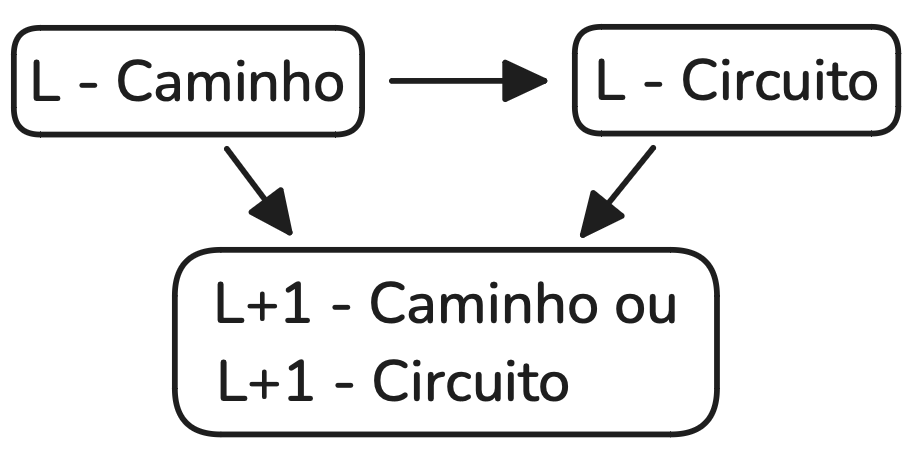
\includegraphics[width=0.8\textwidth]{logos/flowchart.png}
        \captionof{figure}{Fluxograma do algoritmo.}
      \end{center}
      \vspace{1em}

      % \definecolor{shadecolor}{rgb}{0.93, 0.80, 0.82} % pale pink
      % \begin{shaded}
      %   \begin{itemize}
      %     \item[$\bullet$] \textbf{\texttt{create\_union(a, b, t)}}: adiciona a união dos conjuntos que contém $a$ e $b$ no instante de tempo $t$
      %     \item[$\bullet$] \textbf{\texttt{same\_set(a, b, t)}}: consulta se dois elementos pertenciam ao mesmo conjunto no instante $t$
      %     \item[$\bullet$] \textbf{\texttt{delete\_union(t)}}: desfaz a união realizada em $t$
      %   \end{itemize}
      % \end{shaded}
    \end{block}

    \begin{block}{Técnicas utilizadas}
      
      Todas as técnicas utilizam fortemente a condição de Dirac para cada grafo.
      \vspace{1em}

      \textbf{Técnica do cruzamento:}
      
      Seja $P=(x_1, e_1, x_2, \dots, e_{sz}, x_{sz + 1})$, sem repetição de cor e nem de vértice. 
      Suponha que existam duas cores $c_1$ e $c_2$ que não pertencem ao caminho e não existem arestas
      entre $x_1$ e $V \backslash P$ com cor $c_1$ e entre $x_{sz + 1}$ e $V \backslash P$ com cor $c_2$.
      Suponha também que não existe uma aresta de cor $c_1$ ou $c_2$ entre $x_1$ e $x_{sz + 1}$.
      
      Olhando para as arestas de cor $c_1$ que saem de $x_1$, e para as arestas de cor $c_2$ que saem de $x_{sz + 1}$,
      temos que:
      
      $$
        |N_{G_{c_1}}(x_1)| + |N_{G_{c_2}}(x_{sz + 1})| \geq \frac{n}{2} + \frac{n}{2} > sz - 2.
      $$

      Pelo princípio da casa dos pombos, existe um índice $i$ tal que as arestas $(x_1, x_{i+1})$ e $(x_{sz + 1}, x_i)$ são de cores $c_1$ e $c_2$, respectivamente.
      
      Portanto, podemos formar um circuito de tamanho maior como na imagem abaixo:

      \begin{center}
        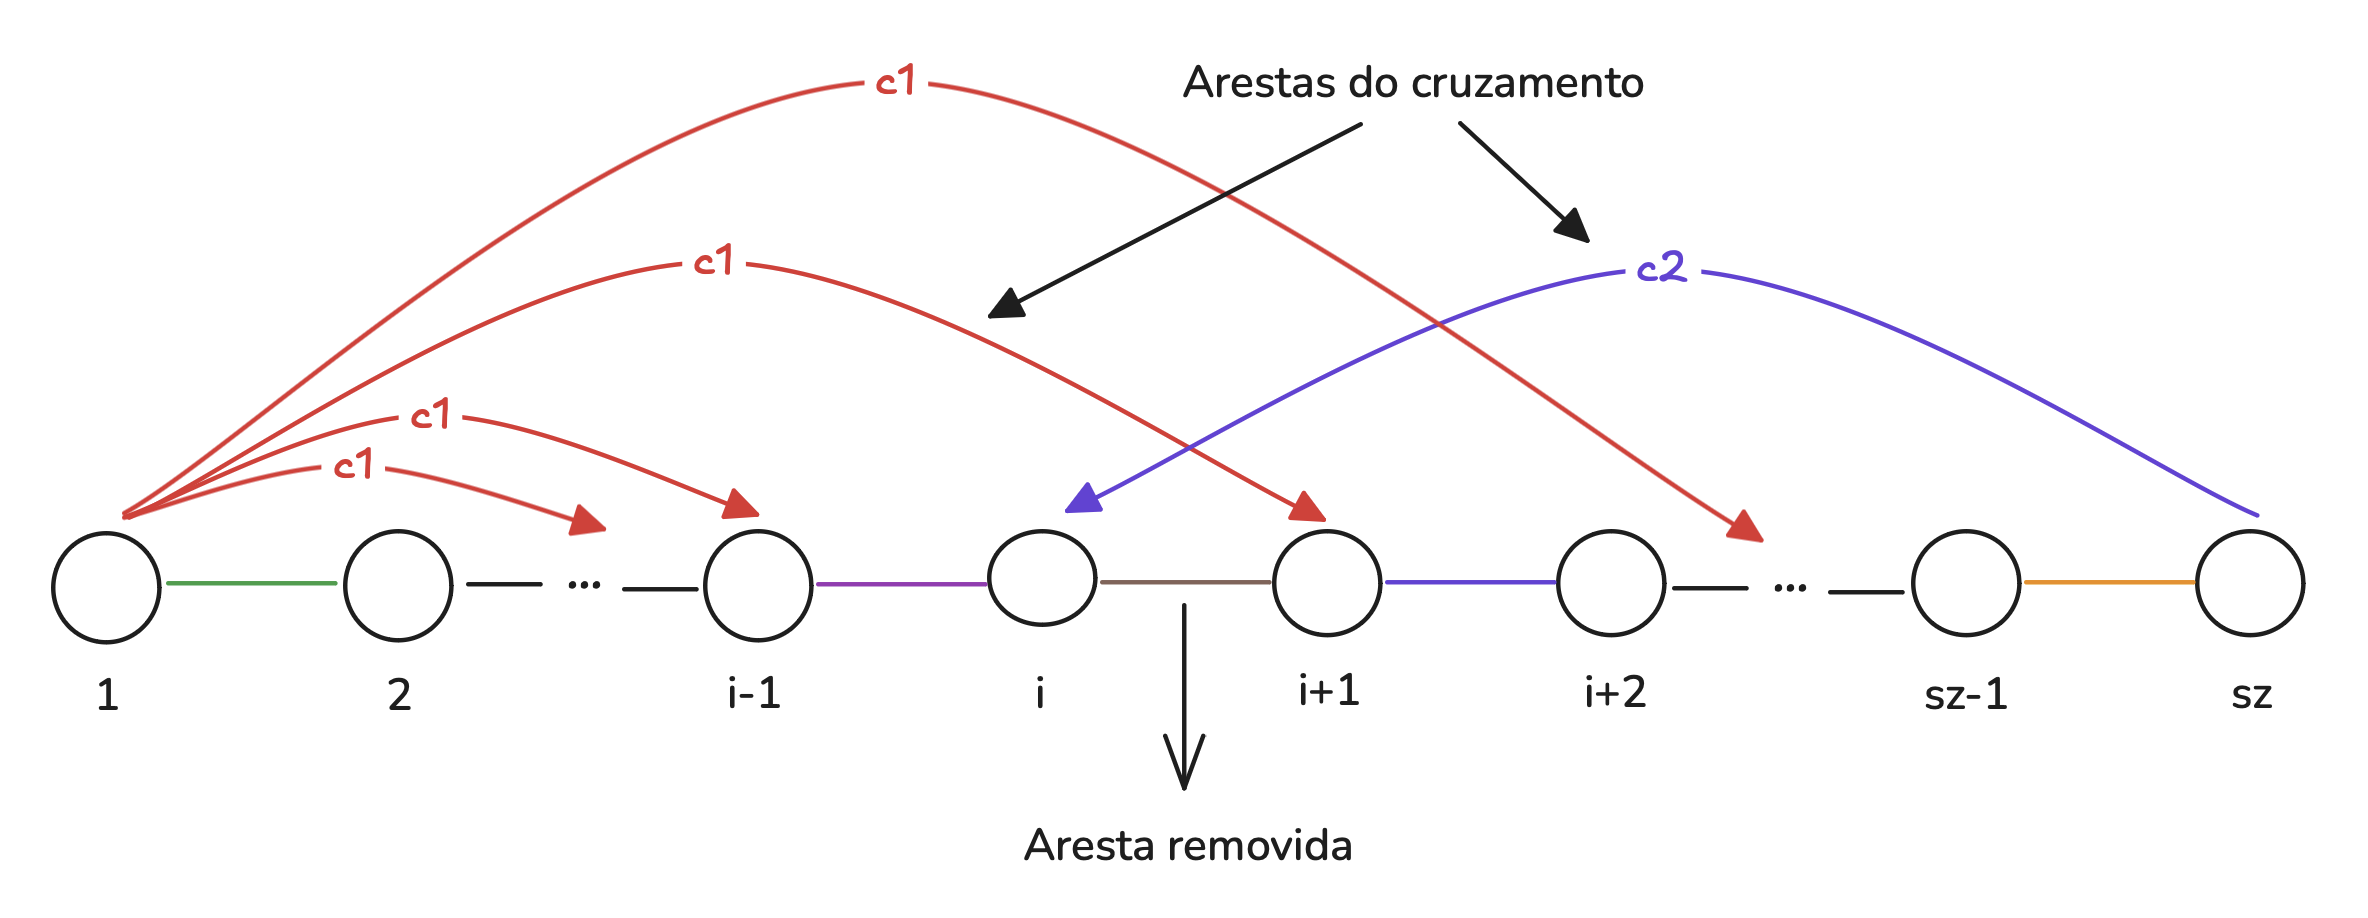
\includegraphics[width=\textwidth]{logos/cruzamento.png}
      \end{center}

    \end{block}


    % ----------------------------------------------------------------------------------------
    % TERCEIRA COLUNA
    % ----------------------------------------------------------------------------------------
    \onethirdcol

    \begin{block}{Implementação}

      A prova feita por \textbf{Joos, Kim (2020)} pode ser adaptada para um algoritmo construtivo, em que o estado é um caminho ou ciclo \textit{rainbow}, e incrementalmente aumentamos o tamanho desse caminho ou ciclo.

      A complexidade do algoritmo é da ordem de $\text{O}(n^3)$, em que $n$ é a ordem de $G$. Essa é complexidade é ótima, pois existem $\text{O}(n^3)$ arestas que devem ser consideradas no input.

      Para validar a corretude da implementação, foram gerados grafos que respeitavam a condição de Dirac com $n$ até $300$;
    \end{block}

  \begin{block}{Animação}

      Animação demonstrando o algoritmo foram feitas com a biblioteca \texttt{manim} (do canal de Youtube \texttt{3Blue1Brown}) em Python. Um exemplo está disponível no QR Code abaixo
      \begin{center}
          
\includegraphics[width=0.5\textwidth]{logos/qrcode.png} 
      \end{center}
  \end{block}


    \begin{block}{Referências}
      As referências estão na página da monografia em \textcolor{jblue}{{\url{https://linux.ime.usp.br/~nathan_luiz}}}
    \end{block}


  \end{columns}
\end{frame}
\end{document}
